% The river model of a black hole. Top: inward flow speed sqrt(rs/r) of the
% river of space against r/rs; it reaches the speed of light at the horizon.
% Bottom: the flow (blue) and the net radial velocity of outgoing light,
% 1 - sqrt(rs/r) (orange), drawn to scale at six radii (arrow length = 0.4 x
% speed, in units of r/rs).
\documentclass[tikz,border=1pt]{standalone}
% Shared preamble for the standalone figures: the book's fonts, palette and
% drawing styles. Figures are drawn at their final printed size. A column is
% 3.35in (241pt) wide; a figure across both columns is 7in (505pt) wide.

\usepackage[T1]{fontenc}
\usepackage{newpxtext}
\usepackage[varbb]{newpxmath}
\usepackage[semibold,scale=0.95,lining]{sourcesanspro}
\usepackage{xcolor}
% Palette shared by the book and by the standalone figures in figures/src.
% One main hue (blue), one accent (orange), and a few roles used sparingly.

\definecolor{seblue}{HTML}{1D5B8F}    % headings, worked examples, main curves
\definecolor{seblueDark}{HTML}{123E63}
\definecolor{seorange}{HTML}{DC7A26}  % thought experiments, light and light cones
\definecolor{seteal}{HTML}{1F8577}    % checks, travellers and ships
\definecolor{sered}{HTML}{C0392B}     % negative energy, tension, violations
\definecolor{seviolet}{HTML}{5E548E}  % going deeper
\definecolor{sesand}{HTML}{8C6A3F}    % history
\definecolor{segray}{HTML}{6B7480}    % axes, guides, secondary labels
\definecolor{selight}{HTML}{D5DAE1}   % grids and faint rules

\usepackage{siunitx}
\usepackage{fontawesome5}
\usepackage{tikz}
\usetikzlibrary{arrows.meta,calc,positioning,decorations.pathreplacing,
  decorations.markings,shapes.geometric,fadings,shadings,patterns,3d,
  intersections,backgrounds}
\usepackage{pgfplots}
\pgfplotsset{compat=1.18}
\usepgfplotslibrary{fillbetween,groupplots,colormaps}

\tikzset{
  >={Latex[length=2.1mm,width=1.4mm]},
  every picture/.style={line cap=round, line join=round},
  lbl/.style={font=\sffamily\footnotesize, text=black!85},
  smalllbl/.style={font=\sffamily\scriptsize, text=black!75},
  guide/.style={segray, line width=0.4pt},
  axisline/.style={segray, line width=0.5pt, -{Latex[length=1.7mm,width=1.1mm]}},
  light/.style={seorange, line width=0.9pt},
  lightdash/.style={seorange, line width=0.9pt, dash pattern=on 3pt off 2pt},
  ship/.style={seteal, line width=1.4pt},
  cone/.style={fill=seorange!22, draw=seorange!85!black, line width=0.35pt},
}

\pgfplotsset{
  se axis/.style={
    axis lines=left,
    axis line style={segray, line width=0.5pt, -{Latex[length=1.6mm,width=1.1mm]}},
    tick style={segray, line width=0.4pt},
    major tick length=2.5pt,
    tick label style={font=\sffamily\scriptsize, text=black!75},
    label style={font=\sffamily\footnotesize, text=black!85},
    every axis plot/.append style={line width=1.1pt},
    legend style={font=\sffamily\scriptsize, draw=none, fill=none},
    scaled ticks=false,
    xticklabel={\sansnum{\tick}}, yticklabel={\sansnum{\tick}},
  },
}

% Numbers in figures are set in the sans-serif text font, with a true minus.
\sisetup{mode=text, reset-text-family=false, reset-text-series=false,
  reset-text-shape=false, drop-zero-decimal, group-minimum-digits=5}
% Tick values arrive as long decimals (1.5000000000); parse them first.
\newcommand{\sansnum}[1]{\begingroup\pgfkeys{/pgf/fpu=false}%
  \pgfmathparse{1*(#1)}\num{\pgfmathresult}\endgroup}

\begin{document}
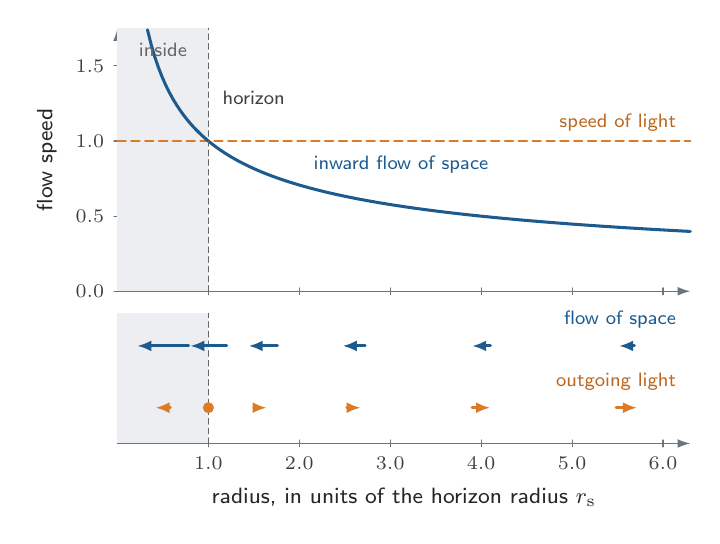
\begin{tikzpicture}
\begin{axis}[
  se axis, name=top,
  width=252pt, height=140pt,
  xmin=0, xmax=6.3, ymin=0, ymax=1.75,
  xtick={1,2,3,4,5,6}, ytick={0,0.5,1,1.5},
  xticklabels={}, ylabel={flow speed},
  clip=false,
]
\fill[selight!45] (axis cs:0,0) rectangle (axis cs:1,1.75);
\draw[seorange, line width=0.8pt, dash pattern=on 3pt off 2pt] (axis cs:0,1) -- (axis cs:6.3,1);
\node[smalllbl, text=seorange!85!black, anchor=south east] at (axis cs:6.25,1.0) {speed of light};
\addplot[seblue, domain=0.33:6.3, samples=150] {sqrt(1/x)};
\node[smalllbl, text=seblue, anchor=south west] at (axis cs:2.05,0.72) {inward flow of space};
\draw[black!60, line width=0.5pt, dash pattern=on 2pt off 1.5pt] (axis cs:1,0) -- (axis cs:1,1.75);
\node[smalllbl, anchor=south west, align=left] at (axis cs:1.05,1.18) {horizon};
\node[smalllbl, text=black!60, anchor=north, align=center] at (axis cs:0.5,1.72) {inside};
\end{axis}
\begin{axis}[
  se axis, at={(top.south west)}, anchor=north west, yshift=-8pt,
  width=252pt, height=92pt,
  xmin=0, xmax=6.3, ymin=-1, ymax=1,
  xtick={1,2,3,4,5,6}, ytick=\empty,
  axis y line=none,
  xlabel={radius, in units of the horizon radius $r_{\mathrm{s}}$},
  clip=false,
]
\fill[selight!45] (axis cs:0,-1) rectangle (axis cs:1,1);
\draw[black!60, line width=0.5pt, dash pattern=on 2pt off 1.5pt] (axis cs:1,-1) -- (axis cs:1,1);
\foreach \r in {0.5,1.0,1.6,2.6,4.0,5.6} {
  \pgfmathsetmacro{\f}{0.4*sqrt(1/\r)}
  \pgfmathsetmacro{\l}{0.4*(1-sqrt(1/\r))}
  \edef\temp{\noexpand\draw[seblue, line width=1.1pt, -{Latex[length=1.8mm,width=1.4mm]}]
    (axis cs:{\r+\f/2},0.5) -- (axis cs:{\r-\f/2},0.5);}\temp
  \ifdim \l pt > 0.01pt
    \edef\temp{\noexpand\draw[seorange, line width=1.1pt, -{Latex[length=1.8mm,width=1.4mm]}]
      (axis cs:{\r-\l/2},-0.45) -- (axis cs:{\r+\l/2},-0.45);}\temp
  \else\ifdim \l pt < -0.01pt
    \edef\temp{\noexpand\draw[seorange, line width=1.1pt, -{Latex[length=1.8mm,width=1.4mm]}]
      (axis cs:{\r-\l/2},-0.45) -- (axis cs:{\r+\l/2},-0.45);}\temp
  \else
    \edef\temp{\noexpand\fill[seorange] (axis cs:\r,-0.45) circle (2pt);}\temp
  \fi\fi
}
\node[smalllbl, text=seblue, anchor=south east] at (axis cs:6.25,0.62) {flow of space};
\node[smalllbl, text=seorange!85!black, anchor=south east] at (axis cs:6.25,-0.33) {outgoing light};
\end{axis}
\end{tikzpicture}
\end{document}
